\chapter{Models}
\label{chapter:models}

In this chapter we present three concrete models, based on the aforementioned theory \todo{right? right?}, which can be applied to protein sequence data. In section \ref{sec:unirep_model} we present the UniRep model, a sequential model based on recurrent neural networks. In section \ref{sec:variational_autoencoder_model} we present a variational auto-encoder working on alignments of protein families. Finally, in section \ref{sec:wavenet_model}, we present the WaveNet model, an autoregressive model which uses convolutional layers to process a protein sequence.% Finally, in section \ref{sec:transformer_model} we present the Transformer, a model based on the idea of attention.

\section{UniRep: A Recurrent Global Model}
\label{sec:unirep_model}
UniRep is a recently proposed protein model that utilizes a recurrent neural network (RNN) to process proteins \cite{alley2019unified}. Because it uses an RNN, it is capable of handling the variable lengths of proteins without needing a sequence alignment. This makes it able to work on global protein space, leading to what the authors of UniRep refers to as a ``unified representation'' -- hence the name.

UniRep works by first embedding each amino acid input sequence to a high-dimensional vector. This sequence of vectors is then fed through a recurrent neural network, producing a sequence of hidden states. The hidden states are then transformed by a linear layer into probabilities for the amino acid following the position of the hidden state. This is illustrated in figure \ref{fig:unirep_architecture}.

The canonical UniRep model presented in \cite{alley2019unified} uses an mLSTM (multiplicative  variant of the common LSTM RNN) with a hidden state size of 1900, as the RNN inside the model. Additionally, it utilizes truncated backpropogation during training.

We have previously worked with UniRep and explored the significance of the above hyperparameters \cite{unirepproject}. We found that the choice of RNN (mLSTM, LSTM or GRU) and the hidden state size is not very significant for performance and one can achieve nearly equivalent performance with a medium-sized LSTM as with the large canonical mLSTM. The choice of RNN and hidden state size can however have a major impact on the computational complexity of the model. We found that truncated backpropogation only made the model perform marginally worse. A diagram of the UniRep model can be seen in figure \ref{fig:unirep_architecture}.

As can be seen in figure \ref{fig:unirep_architecture}, UniRep does not produce a compact, fixed-size representation at any point in its training. This is because UniRep is a sequence-to-sequence model. As such, its representation must be captured externally, after the training is finished. There are many ways one could do this -- in this work, we will use a mean over the RNN's hidden states, which is also what the original UniRep authors proposed.

\begin{figure}[H]
    \centering
    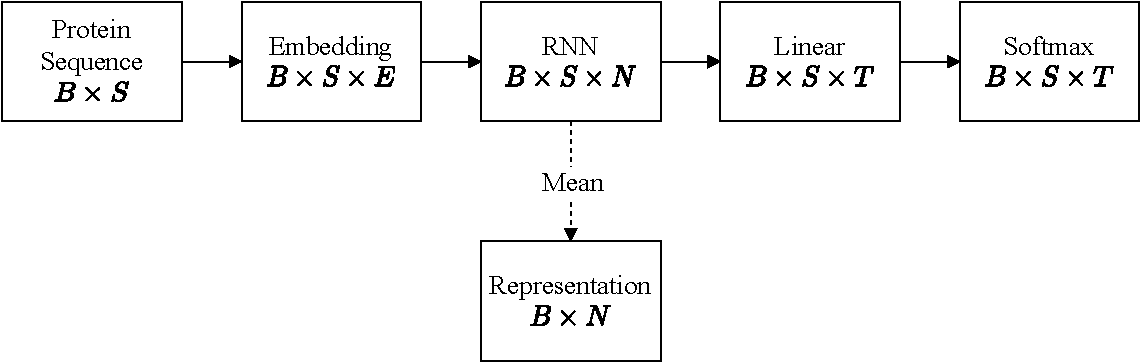
\includegraphics{report/figures/unirep.pdf}
    \caption{Architecture of the UniRep model. $B$ is batch size, $S$ is sequence length, $E$ is the dimension of the embedding layer, $N$ is the size of the RNN's hidden state and $T$ is the number of tokens. UniRep's representation can be obtained by a mean over the RNN's output, but is not used directly in training.}
    \label{fig:unirep_architecture}
\end{figure}

\section{Variational Autoencoder on Aligned Protein Families}
\label{sec:variational_autoencoder_model}

As previously discussed in section \ref{sec:global_local_representations}, producing global representations, meant to be utilized for the entire space of all proteins, may be too optimistic and performance may suffer in the local protein family landscapes. A model constrained to capture representations of a single protein family could be more feasible, because the space of possibilities and variance in the sequences are vastly reduced. Training a model on such a smaller data-set is also simpler, requiring less memory and less time before convergence.

With this in mind, we decided to investigate a model that work on single protein families. There are additional benefits to only working with a single protein family -- it is possible to align the sequences to a single predetermined length. The alignment to a single length allows simple densely connected neural networks to work very effectively on the proteins, since the absoluteness of the sequence positions makes it easy for the weights in the densely connected layers to adjust for each position.

The archetypical variational autoencoder (VAE) uses densely connected neural networks for its encoder and decoder architecture. Also, VAEs have previously been shown to be effective on aligned protein sequence families \cite{riesselman2018deep}. Thus we had good reason to believe that this would be a fruitful experiment.

\subsection{Model Architecture}

In reality, protein sequence positions have a complex interrelated dependency: a single position or groups of positions may have a high determining factor for both specific functionality of the protein and other regions of the sequence. One way to model this otherwise difficult process is to introduce a latent variable and transfer the dependency to that variable. This has the positive effect that it is much easier to model and compute, but also the negative effect that the model is simplified; accounting for all dependencies in a single variable is infeasible.

The evolutionary process of protein generation is modelled by the generative distribution $p(\ve{x}, \ve{z})$ over protein sequences $\ve{x}$ from the space of proteins, and a latent variable $\ve{z}$ that captures the underlying explanatory factors, as described above, and in section \ref{sec:variational_autoencoder}. This includes any dependency between sequence positions, which is important in the calculation of $\pxz$. Specifically, for a protein sequence $\ve{x} = x_1, x_2, \ldots, x_n$ we have $\pxz = \prod_{i = 1}^n p(x_i \mid \ve{z})$, as any dependency between positions have been taken into account by the conditional on $\ve{z}$. Conceptually, this can be thought of as a probabilistic dependency graph, where $\ve{x}$ is separated into its positional dimensions, as shown in figure \ref{fig:codependency}.
\begin{figure}[ht]
    \centering
    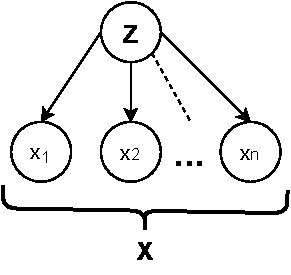
\includegraphics{report/figures/codependency.pdf}
    \caption{The positions $x_1, x_2, \ldots, x_n$ of the sequence $\ve{x}$ are conditionally independent given $\ve{z}$.}
    \label{fig:codependency}
\end{figure}

We model the generating process as $\ve{z}$ causing $\ve{x}$, such that $p\prts{\ve{x}, \ve{z}} = \pxz \pz$.
However, because the involved distributions are unknown, the marginal likelihood $\px$ in equation \ref{eq:marginal_distribution} is inferred, where the average over all latent variables $\ve{z}$ is considered. The encoder produces a likely latent variable $\ve{z}$ given the protein sequence $\ve{x}$ in question. As explained in section \ref{sec:elbo}, training the VAE involves maximizing the ELBO, a lower bound on the log-probability of $\ve{x}$. The VAE is trained to maximize the ELBO; it follows that the ELBO becomes a better approximation of $\log \px$ as the model improves. Thus we can reasonably apply the ELBO as an approximation of $\log \px$.

In order to accomplish the above settings, we constructed a VAE model based on PyTorch's own VAE example\footnote{\url{https://github.com/pytorch/examples/blob/master/vae/main.py}}. We then modified this model, to utilize some of the ideas from \cite{riesselman2018deep}.

For example, we added weights on each sequence, in order to reduce human sampling bias and evolutionary bias, as described in section \ref{sec:bayesian_neural_networks}. These weights are multiplied on the loss for the sequences, and in that way influences how the model weights each sequence in its optimization. Each sequence's weight is calculated as the reciprocal of the number of neighbours the sequence has, where "neighbour" means a sequence within 0.2 Hamming distance.

\todo{write about the dict thing. sparse interactions between positions whatnot}

Another significant deviation from a standard VAE is the addition of Bayesian weights on the linear layers of the decoder. Rather than the decoder using standard deterministic linear layers, it uses probabilistic linear layers. The model samples a weight and bias for the layers every time they are used\footnote{For performance reasons, the model actually samples a single weight and bias for an entire batch.}, instead of having a single deterministic weight and bias. This means that the model optimizes not just a singular linear layer -- instead, it optimizes a distribution of linear layers.

\todo{make figure that shows a linear layer before and after this change. was thinking something like this:}
\begin{figure}[ht]
    \centering
    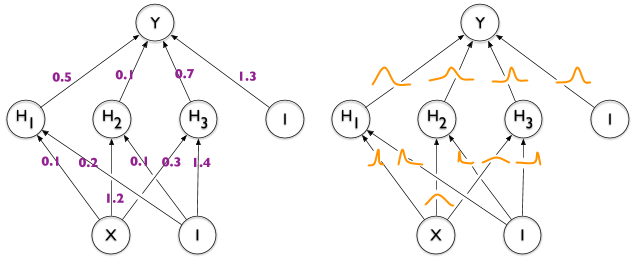
\includegraphics[width = \linewidth]{report/figures/placeholder.png}
    \caption{placeholder \todo{make our own}}
\end{figure}

This distribution of layers is particularly useful at evaluation time. By running the model multiple times on the evaluation data, the model samples different linear layers every time. Effectively, this constructs an ensemble of models of an unlimited size, because the distribution is continuous. Ensembles of models are known to, in general, perform better than single models in isolation. The intuition behind this, is that different models can compensate for each others' weaknesses and shortcomings, thus providing a model that performs better than the mean of the individual models' performances.

% \todo{rethink hyperparameters} We explored various hyperparameters of the model -- the results can be seen in table \ref{tab:vae_hyperparameter_grid}.

% \begin{table}[ht]
%     \centering
%     \begin{tabular}{llll}
%     \hline
%     \textbf{Bayesian/Estimate} & \textbf{Learning rate} & \textbf{Dropout} & \textbf{Spearman $\rho$} \\ \hline
%     Bayesian                   & 0.001                  & 0.0              &                          \\
%     Bayesian                   & 0.001                  & 0.5              &                          \\
%     Bayesian                   & 0.005                  & 0.0              &                          \\
%     Bayesian                   & 0.005                  & 0.5              &                          \\
%     Bayesian                   & 0.0001                 & 0.0              &                          \\
%     Bayesian                   & 0.0001                 & 0.5              &                          \\
%     Estimate                   & 0.001                  & 0.0              &                          \\
%     Estimate                   & 0.001                  & 0.5              &                          \\
%     Estimate                   & 0.005                  & 0.0              &                          \\
%     Estimate                   & 0.005                  & 0.5              &                          \\
%     Estimate                   & 0.0001                 & 0.0              &                          \\
%     Estimate                   & 0.0001                 & 0.5              &                          \\ \hline
%     \end{tabular}
%     \caption{Hyperparameter grid and results for the VAE model.}
%     \label{tab:vae_hyperparameter_grid}
% \end{table}

\section{WaveNet: A Convolutional Model}
\label{sec:wavenet_model}

The \textit{WaveNet} model architechture is a modeling approach similar to UniRep in the sense that it is \textit{autoregressive} and adaptive to unaligned protein sequences \cite{AlQuraishiUnsupervised, oord2016wavenet}. Unlike the variational autoencoder described in section \ref{sec:variational_autoencoder} and \ref{sec:variational_autoencoders_experiement}, the probabilistic model representing the dependencies between amino acid residues is not incorporating a latent variable. Rather, for a protein sequence $\ve{x}_1, \ve{x}_2, \ldots, \ve{x}_n$, the probability of any residue $\ve{x}_i$ is conditioned on the previous residues on the protein chain:
\begin{figure}[H]
    \centering
    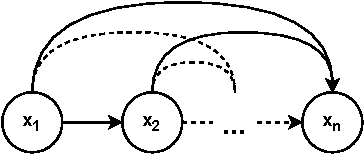
\includegraphics{report/figures/autoregressive.pdf}
    \caption{Caption \todo{caption}}
    \label{fig:autoregressive}
\end{figure}
This is the autoregressive property of the model: each residue is conditioned on the previous residues in the chain. It follows that the probability of the entire protein sequence $\px$ is expressible as a product of the conditioned residue probabilities:
\[ \px = p(\ve{x}_1) \prod_{i = 2}^n p(\ve{x}_i \mid \ve{x}_{i - 1}, \ldots, \ve{x}_1)
\]
\todo{this is actually the same as in unirep, so maybe we should move this to an earlier section} With this setting, the task becomes to model each residue probability, with the restriction that only the previous residues can affect the modeling process. Unlike UniRep, the WaveNet model is not based on recurrent neural networks, but achieves its context by gradually dilating convolution layers, grouped into blocks. A model architecture overview can be seen in figure \ref{fig:wavenet_architecture}.

\begin{figure}[H]
    \centering
    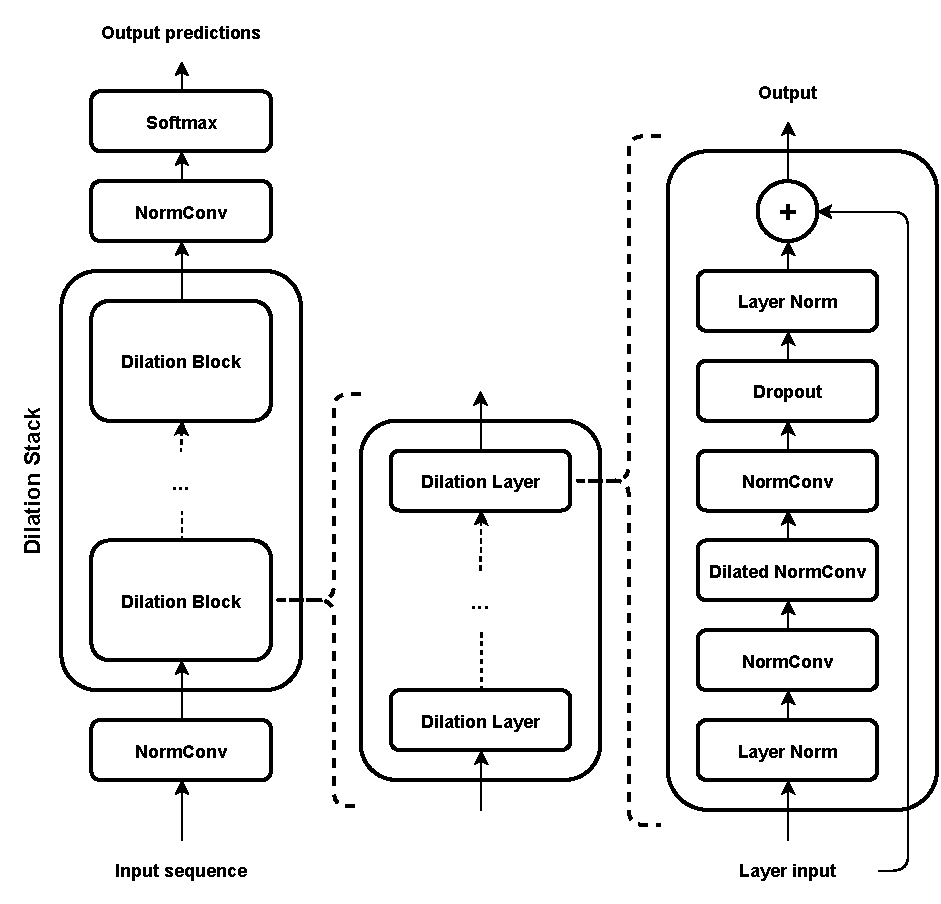
\includegraphics{report/figures/wavenet_architecture.pdf}
    \caption{A WaveNet architecture overview. Model input is passed through a dilation stack (\textit{left}) consisting of dilation blocks. Each dilation block (\textit{middle}) consists of dilation layers. Each dilation (\textit{right}) layer passes its input through a sequence of internal layers.}
    \label{fig:wavenet_architecture}
\end{figure}

The model consists of some core components: the dilation stack, the dilation block and the dilation layer. The dilation stack consists of dilation blocks, which again consists of dilation layers. They all depend on a slightly expanded convolutional layer which we denote as \textit{NormConv}, a contraction of \textit{normalized} and \textit{convolution}. The standard convolutional layer is parameterized by, among other things, the number of in- and out channels, kernel size and a dilation, as discussed in section \ref{sec:convolution}. The NormConv is a standard convolutional with kernel size 1 layer with applied weight normalization\footnote{There are many ways to parameterize equivalent models. In gradient-based optimization, some ways are easier to optimize than others; weight normalization is a procedure to easy optimization by breaking weight parameters into a scale and direction component.} \cite{salimans2016weight} and an additional scale and bias, and potential activation. It returns  an output $\ve{o}$ from an input sample $\ve{x}$ as follows:
\[ \ve{o} = \sigma\prts{\ve{\gamma} \odot \texttt{convolutional}\prts{\ve{x}} + \ve{\beta}}, \]
where $\sigma$ is some activation function, \texttt{convolution} is a standard convolutional layer applied to the input $\ve{x}$, and $\ve{\gamma}$ and $\ve{\beta}$ are learnable parameters that element-wise scale and shift the outcome of the convolution.

The \textit{dilation layer} consists of several internal cells that feed into each other. First, in the \textit{Layer Norm} cell, the input is normalized w.r.t. its empirical mean and variance, and rescaled. Then three Norm Conv layers are applied, where the middle layer is dilated. The dilation depends on the position of the dilation layer in the \textit{dilation block}. For a dilation block of $n$ dilation layers, the dilations are $1, 2, 4, \ldots, 2^n$, so the $i$th dilation layer will have dilation $2^{i - 1}$. All dilated Norm Conv layers have kernel size 2, which in combination with the dilation give rise to the expanding effect of the dilation block, as seen in figure \ref{fig:dilation_layers}. In figure \ref{fig:filters}, three convolution filters that differ in dilation are shown. 

After the Norm Conv layers of the dilation layer, dropout is applied before another layer normalization. The original input to the dilation layer is added to the output of this procedure via a skip connection. This is the output of the dilation layer. The dilation block is many such layers that feed into each other sequentially, and the \textit{dilation stack} is simply many such dilation blocks in sequence. The final output of the dilation stack is passed through a Norm Conv layer that reduces the number of output channels to the number of prediction categories, in our case candidate amino acids.

\begin{figure}[H]
    \centering
    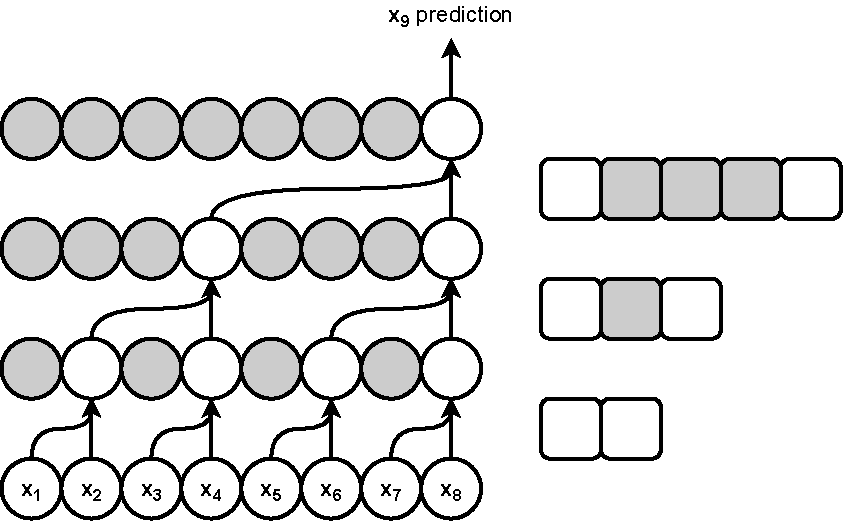
\includegraphics{report/figures/wavenet.pdf}
    \caption{A dilation block with 3 dilation layers with dilation 1, 2 and 4 respectively, in that order, and kernel size 2. The corresponding convolution filters are shown to the right. The the left, the connected nodes show the flow of information from the input sequence, through the dilation layers, to the prediction of the ensuing residual $x_9$.}
    \label{fig:dilation_layers}
\end{figure}

Like the VAE and the UniRep model, WaveNet produces a softmax output over each residue position in the input sequence. In order to to maintain the ordered dependency between residues, any ensuing residues are masked out at each prediction step. That is, for a prediction of the residue at position $i$, the model only observes outcomes from the positions $1, \ldots, i - 1$. This is effectively obtained by shifting the convolution an appropriate number of positions depending on the dilation, and left-padding the sequences.

\todo{change name of model}
\todo{finish this section}
% \todo{result: paper model gets 0.4932 $\rho$ after 25,000 batch updates (size 30) without weights on the samples.}

\subsection{The Causal, Dilated Convolution}
\label{sec:convolution}
A convolutional layer passes its input sequence through a discrete filter and produces output features in size depending on the filter. The convolution filter consists of kernels, which are basically the learnable parameters of the filter. In addition, each filter has a bias parameter. The convolution operation itself is a weighted sum over the input sequence positions under the filter. A \textit{causal} convolution is a convolution which at any position $i$ of the input sequence $x_1, \ldots, x_n$, only considers the $k$ previous positions, where $k$ is the number of kernels in the filter. That is, at position $i$, the convolution operation is $b + \sum_{m=1}^k f_m \cdot x_{i - k + m}$, where $f_m$ is the $m$th filter kernel and $b$ is a bias parameter. See figure \ref{fig:convolution} for an example.

\begin{figure}[H]
    \centering
    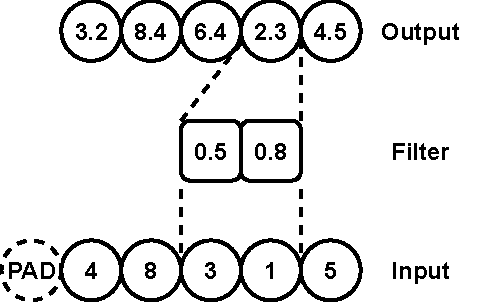
\includegraphics{report/figures/convolution.pdf}
    \caption{Example of a one-dimensional causal convolution using a filter with 2 kernels and no bias. The input sequence is right-padded to maintain the same output length as the input. The causal relation is from left to right. Here, $f_1 = 0.5$ and $f_2 = 0.8$. At the shown output node, the convolution calculation is $0.5 \cdot 3 + 0.8 \cdot 1 = 2.3$.}
    \label{fig:convolution}
\end{figure}

In addition, a convolution can be \textit{dilated}, meaning that the filter kernels are not applied to adjacent positions in the input sequence, but separated by a number of intermediate positions. An example operation similar to figure \ref{fig:convolution} is shown in figure \ref{fig:dilated_convolution}. Three different dilation filters are shown in figure \ref{fig:filters}.

\begin{figure}[H]
    \centering
    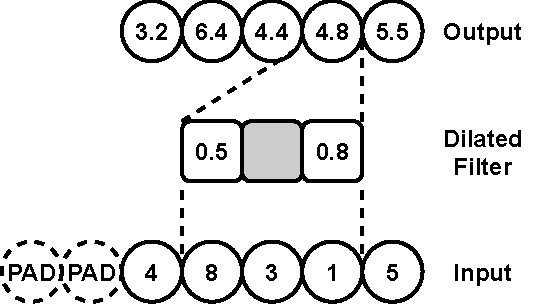
\includegraphics{report/figures/dilated_convolution.pdf}
    \caption{A one-dimensional \textit{dilated} causal convolution using a filter with 2 kernels, dilation 2 and no bias. The input sequence is right-padded to maintain the same output length as the input. The causal relation is from left to right. At the shown output node, the convolution calculation is $0.5 \cdot 8 + 0 \cdot 3 + 0.8 \cdot 1 = 4.8$.}
    \label{fig:dilated_convolution}
\end{figure}

\begin{figure}[H]
    \centering
    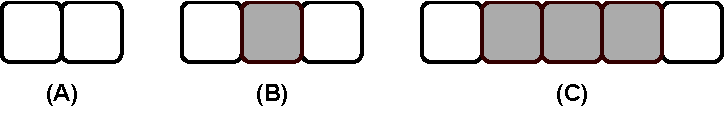
\includegraphics{report/figures/filters.pdf}
    \caption{Three one-dimensional convolution filters with kernel size 2. White boxes denote positions that are weighted in the convolution. Shaded boxes are skipped/masked. (A) dilation of 1. (B) dilation of 2. (C) dilation of 4.}
    \label{fig:filters}
\end{figure}

A convolution layer is typically parameterized with a number of filters, determining the number of \textit{output channels}. For input sequences where each position is multi-dimensional, the convolution filters are shaped accordingly. The dimensionality of the input positions is called the number of \textit{input channels}. Each filter reduces every position to a scalar. By applying a number of filter, the desired output channel can be achieved. The number of weights of the convolution layer will then be \texttt{input channels} $\times$ \texttt{kernels} $\times$ \texttt{output channels}.

\todo{write about ensemble. write why it makes sense to make an ensemble: bias-variance tradeoff.}

%\section{The Transformer: An Attention-based Model}
%\label{sec:transformer_model}
%The final model that we will consider is the Transformer \cite{vaswani2017attention}. The Transformer is based on the idea of attention, which is a technique used with sequential models (classically recurrent neural networks). Intuitively, an attention mechanism attempts to learn which parts of the input to ``pay attention to'' when decoding the output sequence. For example, in a natural language setting, this can be useful to disambiguate what previously mentioned subject a pronoun refers to, which makes a model much better at reading comprehension. In the protein setting, one would hope that the attention mechanism would learn which amino acids of the protein to pay attention to -- this could for example be the amino acids that are spatially close to the decoded amino acid, thus giving the model a way to account for physical contact between the protein itself.
%
%The Transformer model has been shown to be incredibly effective in natural language processing, giving rise to models which can produce text that appears as though it was written by a human \todo{cite GPT, GPT-2 or Bert or something}. In section \ref{sec:transformer_experiment} we would like to explore whether it can also be effective when working on proteins.
%
%The Transformer is a model capable of working on sequences, but it is not a sequential model per se. That is, it does not process one element of the input sequence at a time, unlike a recurrent neural network. Rather, it processes all the elements of the input sequence in parallel, which helps to improve the performance of the model, but also alleviate some of the problems with RNNs long computation graphs, that is, vanishing and exploding gradients.
%
%However, this lack of sequential processing means that the Transformer does not inherently know its position in the sequence when decoding. In order to give this information to the Transformer, one must use an embedding of the sequence elements. Consider a sequence $S = \crts{s_1, \dots, s_n}$. Typically, two methods of embedding the sequence elements are employed: learnable embedding and positional embedding. 
%
%A learnable embedding is simply a one-to-one mapping from sequence elements to high-dimensional vectors. In natural language processing, words are usually embedded to vectors with hundreds of dimensions, since there are so many different words. Comparatively, there are merely 20 or so amino acids, so fewer dimensions can suffice in this case. Actually, a simple one-hot encoding might even suffice, though this does not allow us to learn the embedding (which could be useful).
%
%A positional embedding is a special kind of embedding employed with the Transformer in order to inform the model of its current position in the sequence. Basically, the positional embedding is a ``fingerprint'' of where the element resides in the sequence. Usually, a mix of sine curves are used as this fingerprint. A positional embedding can be utilized at the same time as a learnable embedding or with a one-hot encoding, by simply summing or concatenating the two embeddings.
%
%\todo{something something transformer is not an autoregressive model either}
%
%The Transformer architecture consists of a mix of linear layers and so-called ``multi-head self-attention''. ``Self-attention'' signifies that this is a special kind of attention mechanism, while ``multi-head'' refers to the way the attention mechanism is performed multiple times and then combined to obtain the output.
%
%Consider an input sequence $X = \crts{x_1, \dots, x_n}$ where each $x_i$ is an embedded vector as described above. The self-attention mechanism calculates a weight (or ``attention'', if you will) for each pair $(x_i, x_j)$ of $X$. This weight is multiplied on $x_j$ and the resulting weighted sequence elements are summed to produce an output for $x_i$. Concretely, the calculation is done using matrices. Let $\mat{X}$ be a 2D matrix where row $i$ equals $x_i$. Then the output $\mat{Z}$ is calculated like so \cite{illustrated_transformer}:
%\begin{align*}
%    \mat{Q} &= \mat{X} \mat{W}_Q \\
%    \mat{K} &= \mat{X} \mat{W}_K \\
%    \mat{V} &= \mat{X} \mat{W}_V \\
%    \mat{S} &= \sigma\prts{\frac{\mat{Q} \mat{K}^T}{\sqrt{d_k}}} \\
%    \mat{Z} &= \mat{S} \mat{V}
%\end{align*}
%Where $Q$ is known as the query matrix, $K$ as the key matrix and $V$ as the value matrix. $\mat{W}_Q$, $\mat{W}_K$ and $\mat{W}_V$ are learnable parameters. $\mat{S}$ contains the score for each pair of elements in $X$, $\sigma$ is the softmax function and $d_k$ is the number of columns in the $\mat{W}_K$ matrix. Finally, $\mat{Z}$ is the output of the self-attention layer. In \textit{multi-head} self-attention, the Transformer will have $m$ self-attention layers, each producing a $\mat{Z}_i$. All of the $\mat{Z}_i$s are concatenated and the result is multiplied by another learnable parameter $\mat{W}_O$:
%\[\mat{O} = \prts{\mat{Z}_1 \oplus \mat{Z}_2 \oplus \dots \oplus \mat{Z}_m} \mat{W}_O\]
%Where $\oplus$ indicates concatenation along the horizontal axis. This final result $\mat{O}$ is then put through some linear layers, producing the final output sequence.
